\section{Solvers for SDEs}
We consider now stochastic differential equations in the form
\begin{equation} \label{4_problem}
    dx(t) = f(t,x(t),p_f) dt + g(t,x(t),p_g) d\omega (t), \hspace{1em} d \omega (t) \sim \mathcal{N}_{iid}(0, Idt)
\end{equation}
where $x \in \mathbb{R}^{n_x}$ and $\omega$ is a stochastic variable with dimension $n_w$, $p_f$ and $p_g$ are parameters for $f:\mathbb{R} \times \mathbb{R}^{n_x} \times \mathbb{R}^{n_{p_f}} \to \mathbb{R}^{n_x}$ and $g:\mathbb{R} \times \mathbb{R}^{n_x} \times \mathbb{R}^{n_{p_g}} \to \mathbb{R}^{n_x \times n_w}$ (i.e. the result of $g$ is a matrix of size $n_x \times n_w$).

\subsection{Make a function in Matlab that can realize a multivariate standard Wiener process.}
We implement the Wiener process in the following function. This generates \code{Ns} realizations of a Wiener process of size \code{nW}.

\begin{lstlisting}[caption = Multivariate standard Wiener process, captionpos=b, label=4_wiener]
function [Tw,W,dW] = StdWienerProcess(tspan,h,nW,Ns,seed)

if nargin == 4
    rng(seed);
end

t0 = tspan(1);
tf = tspan(2);

Tw = t0:h:tf;
N = size(Tw,2);

dW = sqrt(h)*randn(nW,N,Ns);
W  = [zeros(nW,1,Ns) cumsum(dW,2)];
W = W(:,1:end-1,:);
end

\end{lstlisting}
\subsection{Implement the explicit-explicit method with fixed step size.}
\begin{lstlisting}[caption = Euler-Maruyama Method, captionpos=b, label=4_EulerMaruyama]
function [T,X] = EulerMaruyama(ffun,gfun,tspan,h,x0,nW,args)
t0 = tspan(1);
tf = tspan(end);
T = t0:h:tf;
N  = size(T,2);

X  = zeros(size(x0,1),N);
X(:,1) = x0;

[~,~,dW] = StdWienerProcess(tspan,h,nW,1);

for k=1:N-1
    f = feval(ffun,T(k),X(:,k),args{:});
    g = feval(gfun,T(k),X(:,k),args{:});

    psi = X(:,k) + g*dW(:,k);

    X(:,k+1) = psi + h*f;
end

\end{lstlisting}

\pagebreak

\subsection{Implement the implicit-explicit method with fixed step size.}
\begin{lstlisting}[caption = Newton's Method for SDEs, captionpos=b, label=4_NewtonsMethodSDE]
function [x,f,J] = NewtonsMethodSDE(ffun,t,h,psi,xinit,tol,maxit,args)
I = eye(length(xinit));
x = xinit;

[f,J] = feval(ffun,t,x,args{:});
R = x - h*f - psi;
it = 1;

while ( (norm(R,'inf')>tol) &&(it<= maxit) )
    dRdx = I - J*h;
    mdx = dRdx\R;

    x   = x - mdx;
    [f,J] = feval(ffun,t,x,args{:});
    R = x - h*f - psi;
    it = it + 1;
end
end
\end{lstlisting}

\begin{lstlisting}[caption = Implicit-Explicit Method, captionpos=b, label=4_ImplicitExplicit]
function [T,X] = ImplicitExplicit(ffun,gfun,tspan,h,x0,nW,args)

newtontol = 1e-8;
maxit = 100;

t0 = tspan(1);
tf = tspan(end);
T = t0:h:tf;
N  = size(T,2);

X  = zeros(size(x0,1),N);
X(:,1) = x0;

[~,~,dW] = StdWienerProcess(tspan,h,nW,1);
k = 1;

f = feval(ffun,T(k),X(:,k),args{:});
for k=1:N-1
    g = feval(gfun,T(k),X(:,k),args{:});

    psi = X(:,k) + g*dW(:,k);

    xinit = psi + h*f;
    [X(:,k+1),f,~] = NewtonsMethodSDE(ffun,T(:,k+1),h,psi,xinit,newtontol,maxit,args);
end
end

\end{lstlisting}

\subsection{ Describe your implementations and the idea you use in deriving the methods.  Provide Matlab code for your implementations.}
The idea behind the Euler-Maruyama and Implicit-Explicit is the same as in the Explicit and Implicit Euler already described in Parts \ref{part2} and \ref{part3}, for the function $f$. The problem is that now we also have a function $g$ associated to the Wiener process and, as in order to calculate it we need to discretize it, we just use the Explicit Euler for $g$ both in Euler-Maruyama and Implicit-Explicit. Notice that the Newton's method for SDEs is slightly different to the one already presented in Listing \ref{3_NewtonsMethod}. The Matlab code is already provided in the last two questions.

\pagebreak

\subsection{Test your implementations using SDE versions of the Van der Pol problem.}
We will test the implementations in two SDE versions of the Van der Pol problem. One with \textit{state independent diffusion}:
\begin{align*}
    dx_1(t) &= x_2(t)dt, \\
    dx_2(t) &= \left[ \mu (1-x_1(t)^2)x_2(t) - x_1(t) \right] dt + \sigma d\omega (t),
\end{align*}
and another one with \textit{state dependent diffusion}:
\begin{align*}
    dx_1(t) &= x_2(t)dt, \\
    dx_2(t) &= \left[ \mu (1-x_1(t)^2)x_2(t) - x_1(t) \right] dt + \sigma(1+x_1(t)^2) d\omega (t).
\end{align*}

We implement $f$ and the two $g$s in the following scripts:
\begin{lstlisting}
function [f,J] = VanderPolDrift(t,x,mu,sigma)
f = zeros(2, 1);

f(1) = x(2);
f(2) = mu * (1 - x(1)^2)*x(2) - x(1);

if nargout > 1
    J = zeros(2, 2);

    J(1,2) = 1;
    J(2,1) = -2 * mu * x(1) * x(2) - 1;
    J(2,2) = mu * (1-x(1)^2);
end
end

function g = VanderPolDiffusion1(t,x,mu,sigma)
g = [0; sigma];
end

function g = VanderPolDiffusion2(t,x,mu,sigma)
g = [0; sigma*(1.0+x(1)^2)];
end
\end{lstlisting}

In the following plots we show 5 realisations of the Euler-Maruyama and the Implicit-Explicit methods for the state independent diffusion case ($\sigma=1$) and for the dependent ($\sigma=0.5$). The runs were obtained setting $\mu = 3$, $h=0.1$, $\code{tspan} = [0,40]$ and $x_0 = [0.5;0.5]$.

\begin{figure}[H]
    \centering
    \makebox[\textwidth][c]{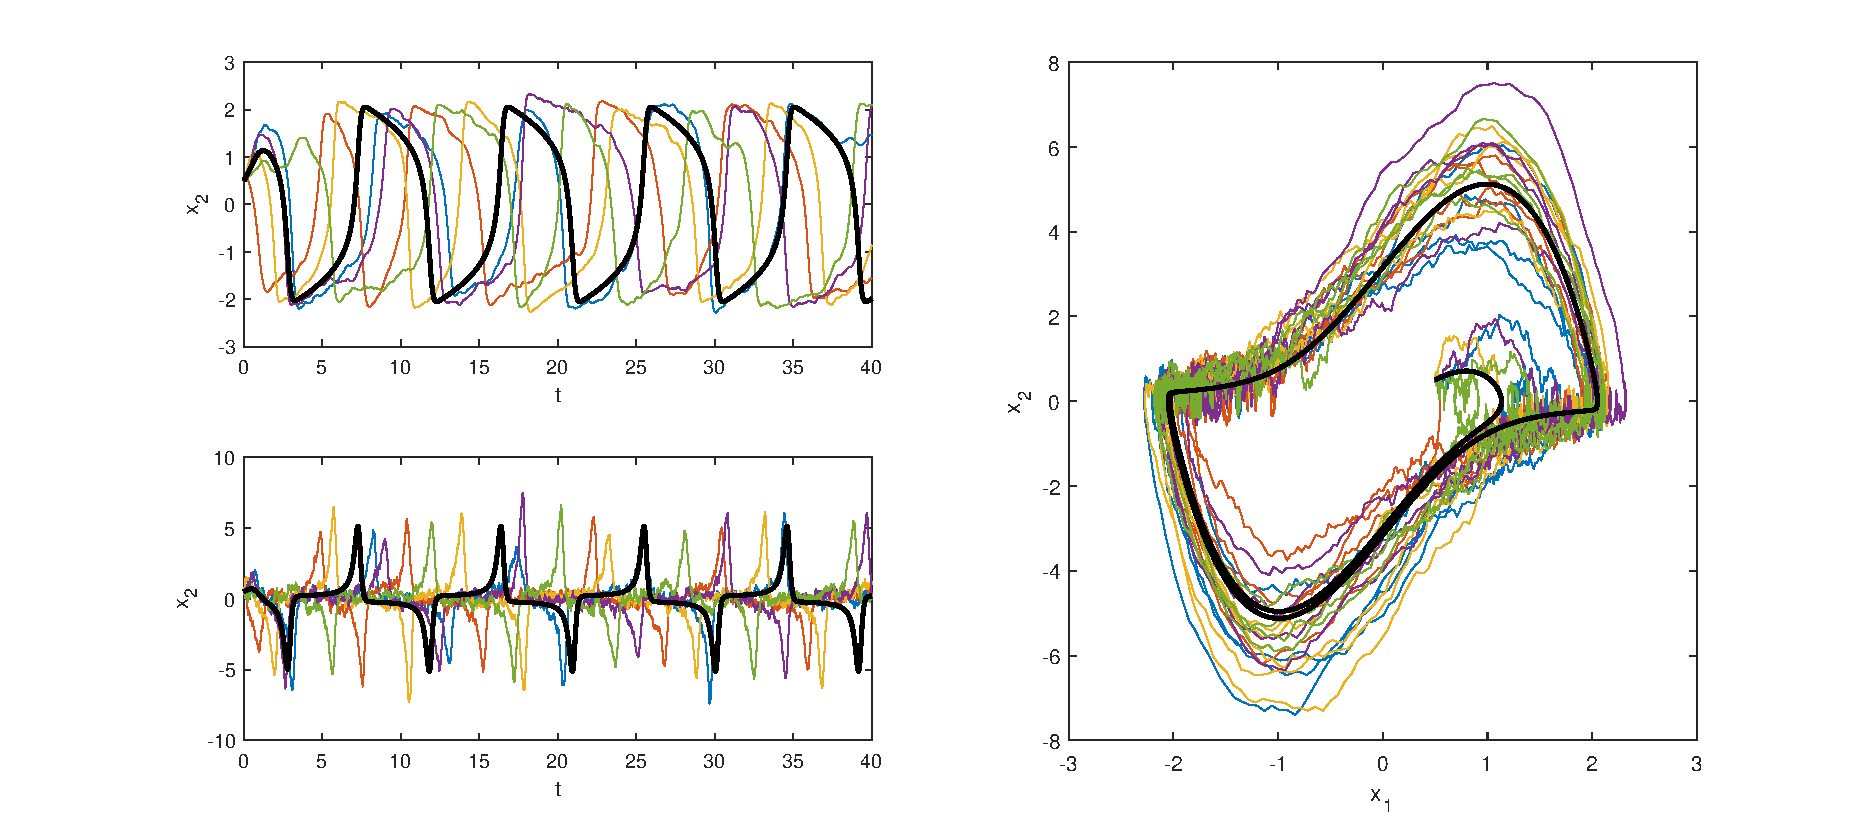
\includegraphics[width=1.25\textwidth]{images/4/4_5_EulerMaruyama_independent.pdf}}
    \caption{5 realisations of the solution for the Van der Pol SDE problem with state independent diffusion ($\mathit{\mu = 3, \sigma=1}$) using Euler-Maruyama with fixed step size}
    \label{4_5_EulerMaruyama_Independent}
\end{figure}

\begin{figure}[H]
    \centering
    \makebox[\textwidth][c]{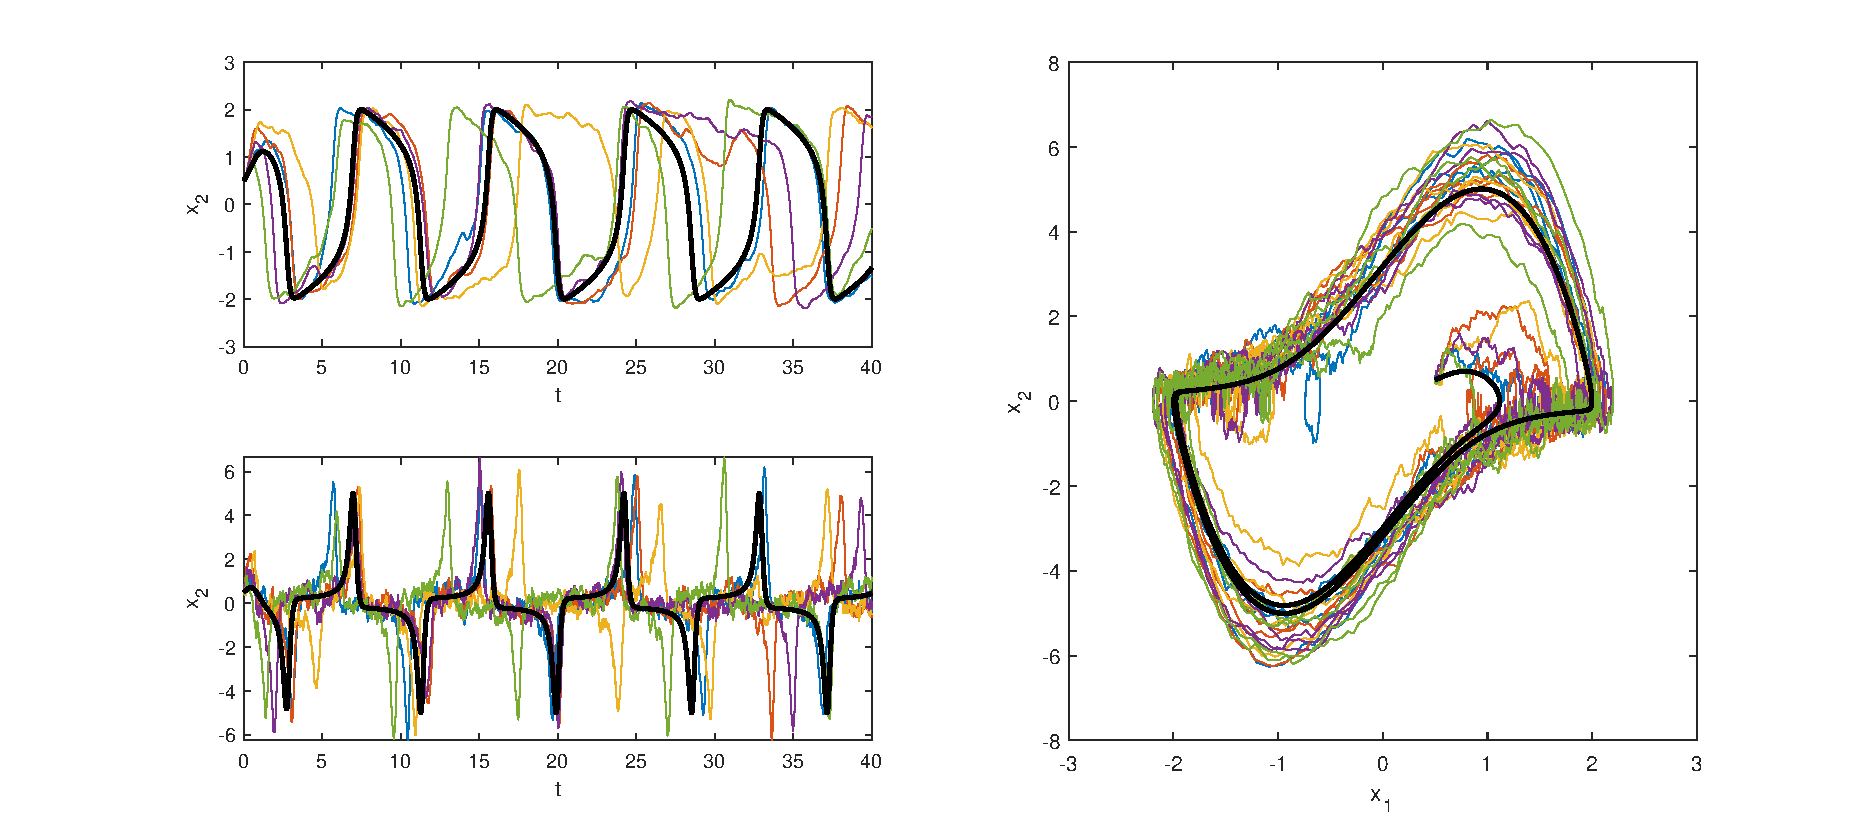
\includegraphics[width=1.25\textwidth]{images/4/4_5_ImplicitExplicit_independent.pdf}}
    \caption{5 realisations of the solution for the Van der Pol SDE problem with state independent diffusion ($\mathit{\mu = 3, \sigma=1}$) using Implicit-Explicit with fixed step size}
    \label{4_5_ImplicitExplicit_Independent}
\end{figure}

\begin{figure}[H]
    \centering
    \makebox[\textwidth][c]{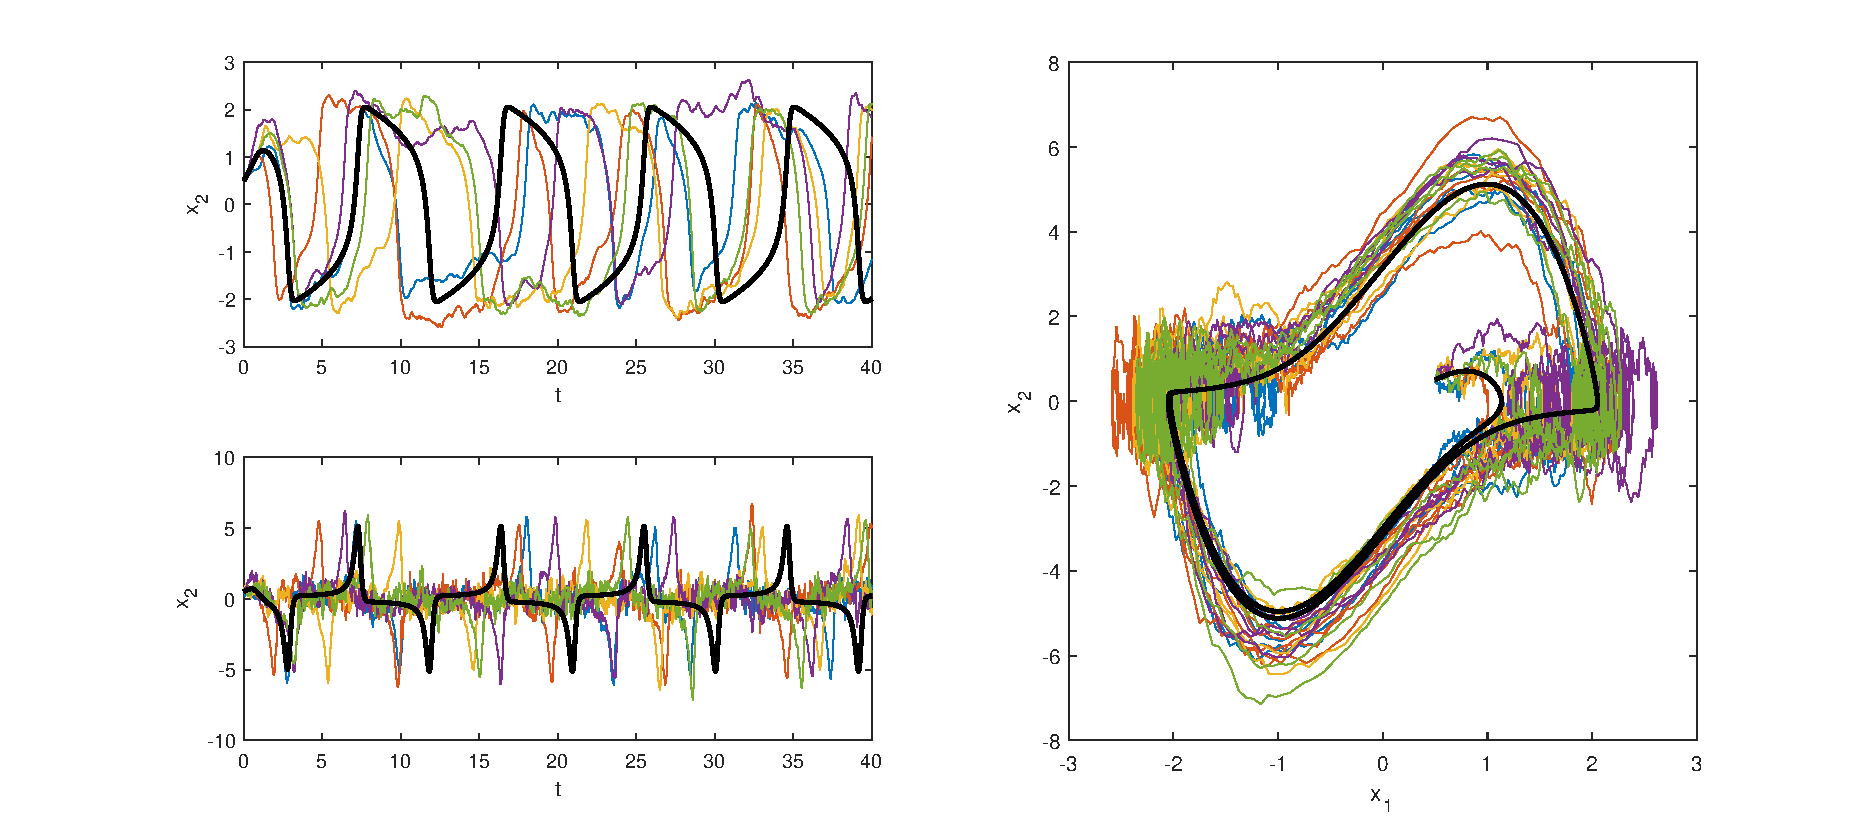
\includegraphics[width=1.25\textwidth]{images/4/4_5_EulerMaruyama_dependent.pdf}}
    \caption{5 realisations of the solution for the Van der Pol SDE problem with state dependent diffusion ($\mathit{\mu = 3, \sigma=0.5}$) using Euler-Maruyama with fixed step size}
    \label{4_5_EulerMaruyama_dependent}
\end{figure}

\begin{figure}[H]
    \centering
    \makebox[\textwidth][c]{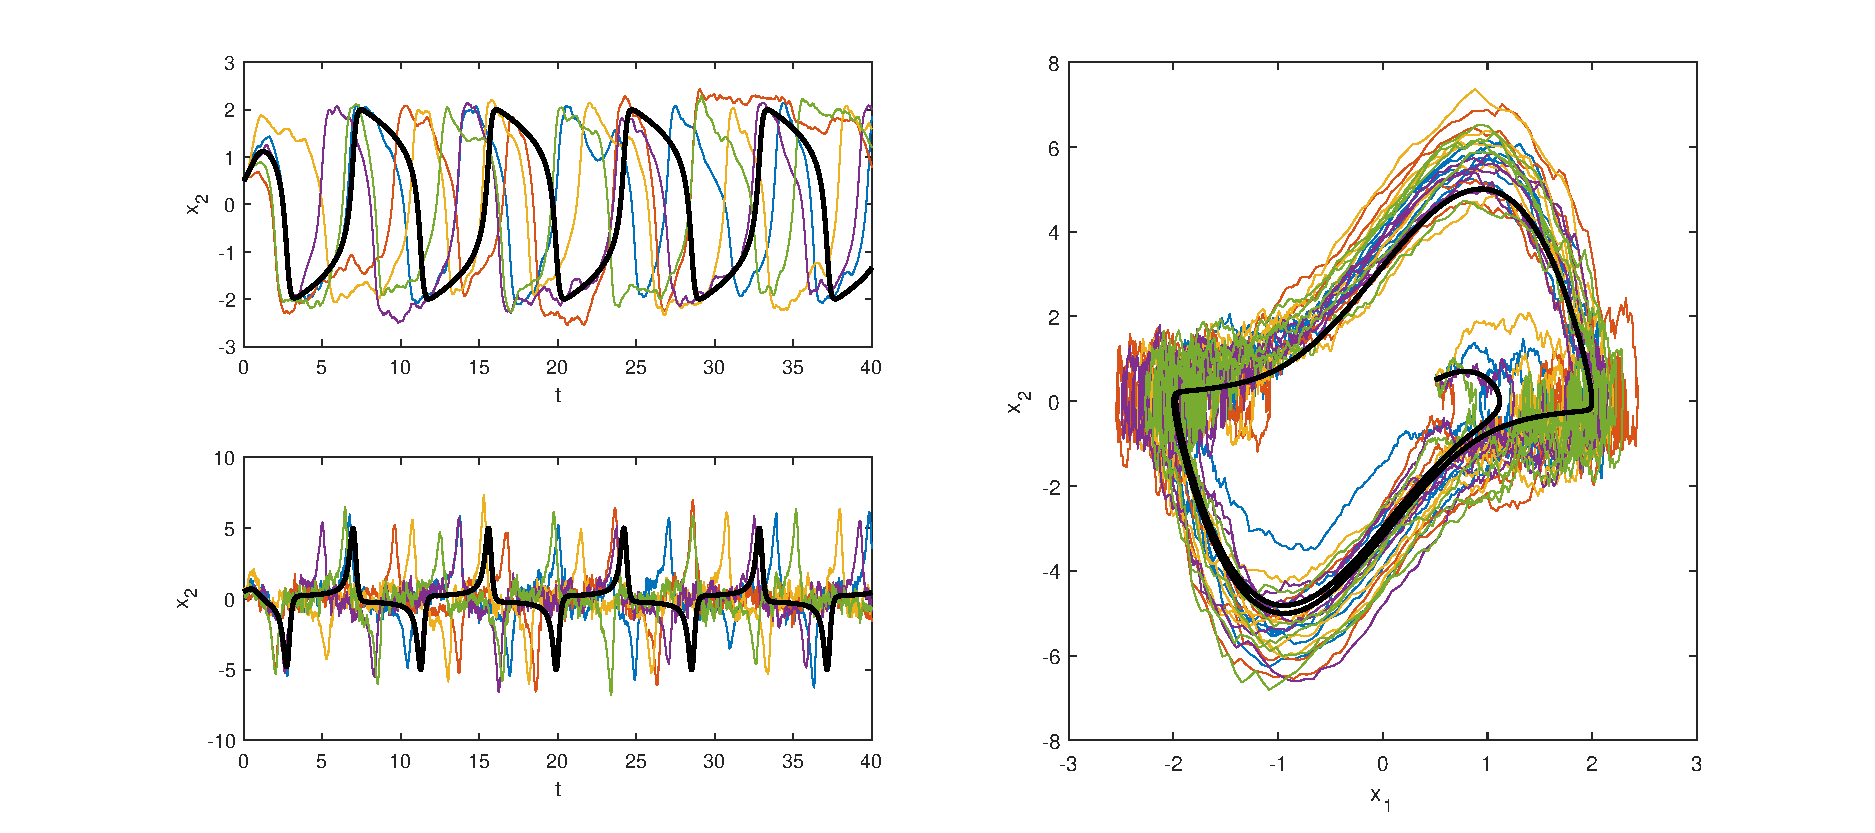
\includegraphics[width=1.25\textwidth]{images/4/4_5_ImplicitExplicit_dependent.pdf}}
    \caption{5 realisations of the solution for the Van der Pol SDE problem with state dependent diffusion ($\mathit{\mu = 3, \sigma=0.5}$) using Implicit-Explicit with fixed step size}
    \label{4_5_ImplicitExplicit_dependent}
\end{figure}

\subsection{Test  your  algorithms  on  the  adiabatic  CSTR  problem  described  in  the papers uploaded to Learn (3D-version and 1D-version).}
For the CSTR problem, we'll also compute 5 realisations of the Euler-Maruyama and the Implicit-Explicit  methods for the 3D and the 1D case. These runs are obtained setting all the parameters as in \cite{Bagterp1} and \cite{Bagterp2}. $\sigma$ was set to $0.5$ for all runs. It's worth noticing how the noise decreases for the 1D problem even though they are run with the same $\sigma$.

\vspace{3cm}

\begin{figure}[H]
\centering
    \begin{subfigure}{0.8\linewidth}
        \centering
        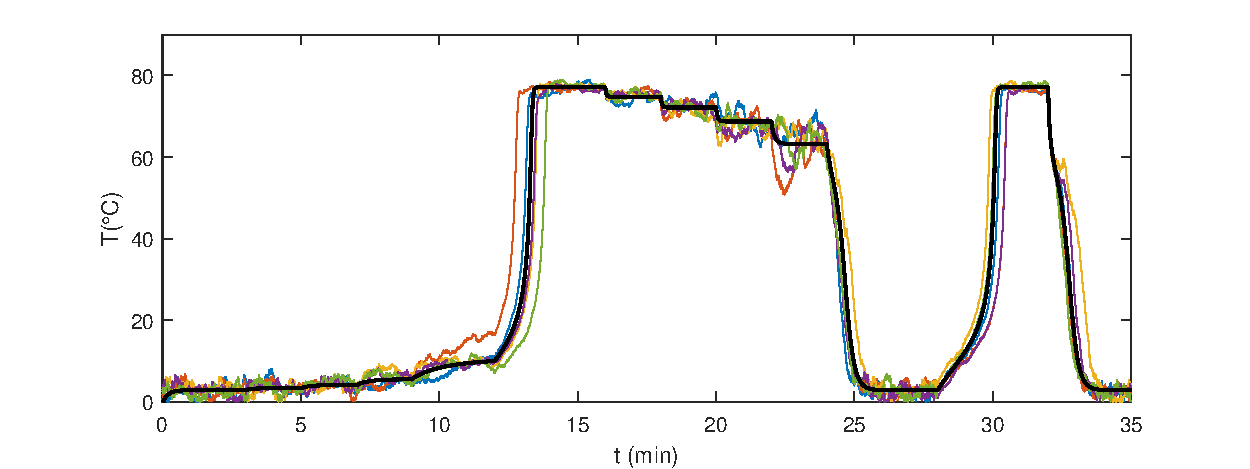
\includegraphics[width=1\linewidth]{images/4/4_6_EulerMaruyama_3D.pdf} 
        \caption{Euler-Maruyama method}
    \end{subfigure} \\
    \begin{subfigure}{0.8\linewidth}
        \centering
        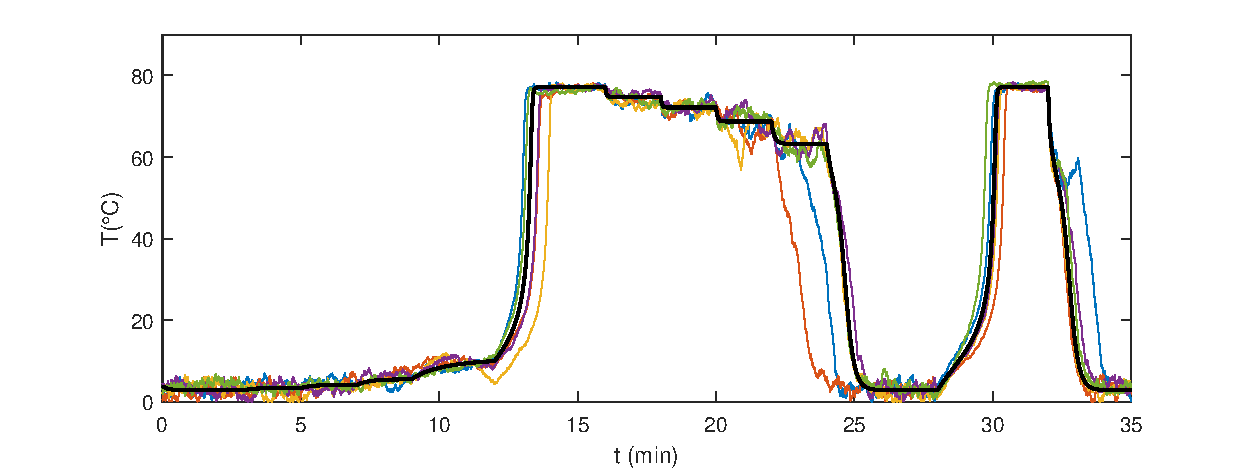
\includegraphics[width=1\linewidth]{images/4/4_6_ImplicitExplicit_3D.pdf}
        \caption{Implicit-Explicit method}
    \end{subfigure}
    \caption{5 realisations of the solution for the 3D CSTR SDE problem ($\sigma = 5$) using fixed step size}
    \label{4_6_EM_vs_IE_3D}
\end{figure}

\vspace{5cm}

\begin{figure}[p]
\centering
    \begin{subfigure}{0.8\linewidth}
        \centering
        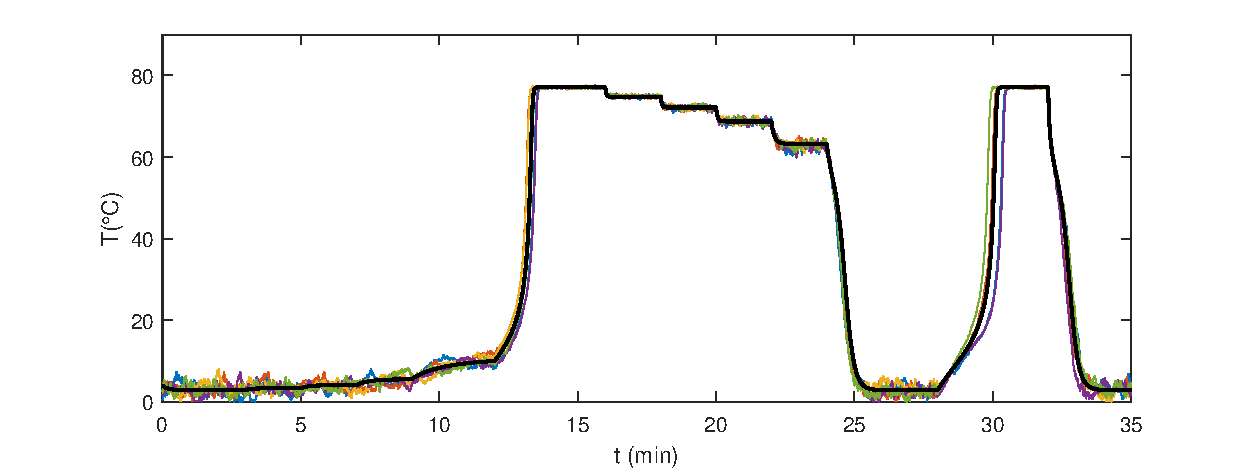
\includegraphics[width=1\linewidth]{images/4/4_6_EulerMaruyama_1D.pdf} 
        \caption{Euler-Maruyama method}
    \end{subfigure} \\
    \begin{subfigure}{0.8\linewidth}
        \centering
        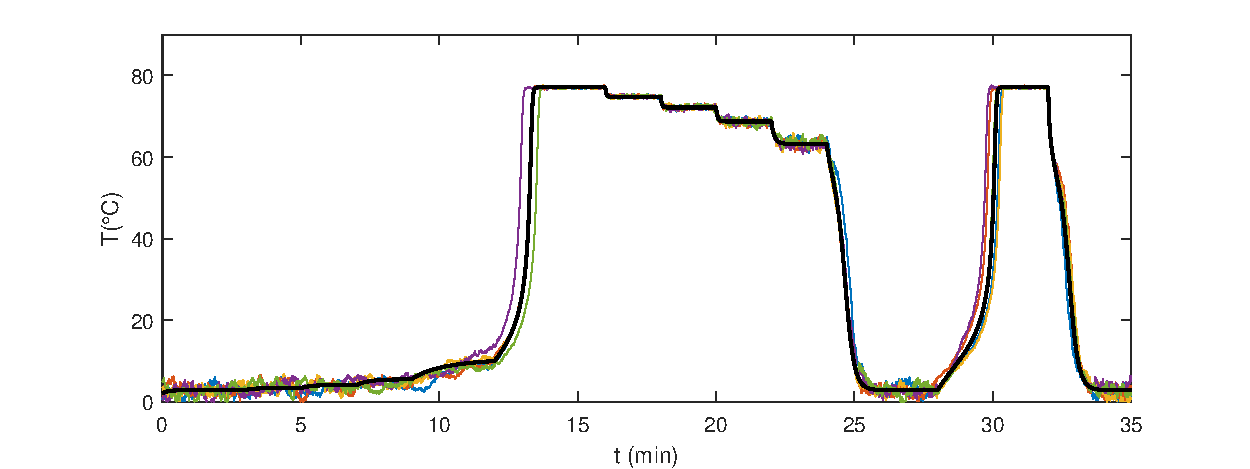
\includegraphics[width=1\linewidth]{images/4/4_6_ImplicitExplicit_1D.pdf}
        \caption{Implicit-Explicit method}
    \end{subfigure}
    \caption{5 realisations of the solution for the 1D CSTR SDE problem ($\sigma = 5$) using fixed step size}
    \label{4_6_EM_vs_IE_1D}
\end{figure}